\appendix
\section{Appendix: Count rates and acceptances for the "FT" and "no-FT" configurations}
\begin{figure}  
\begin{center}
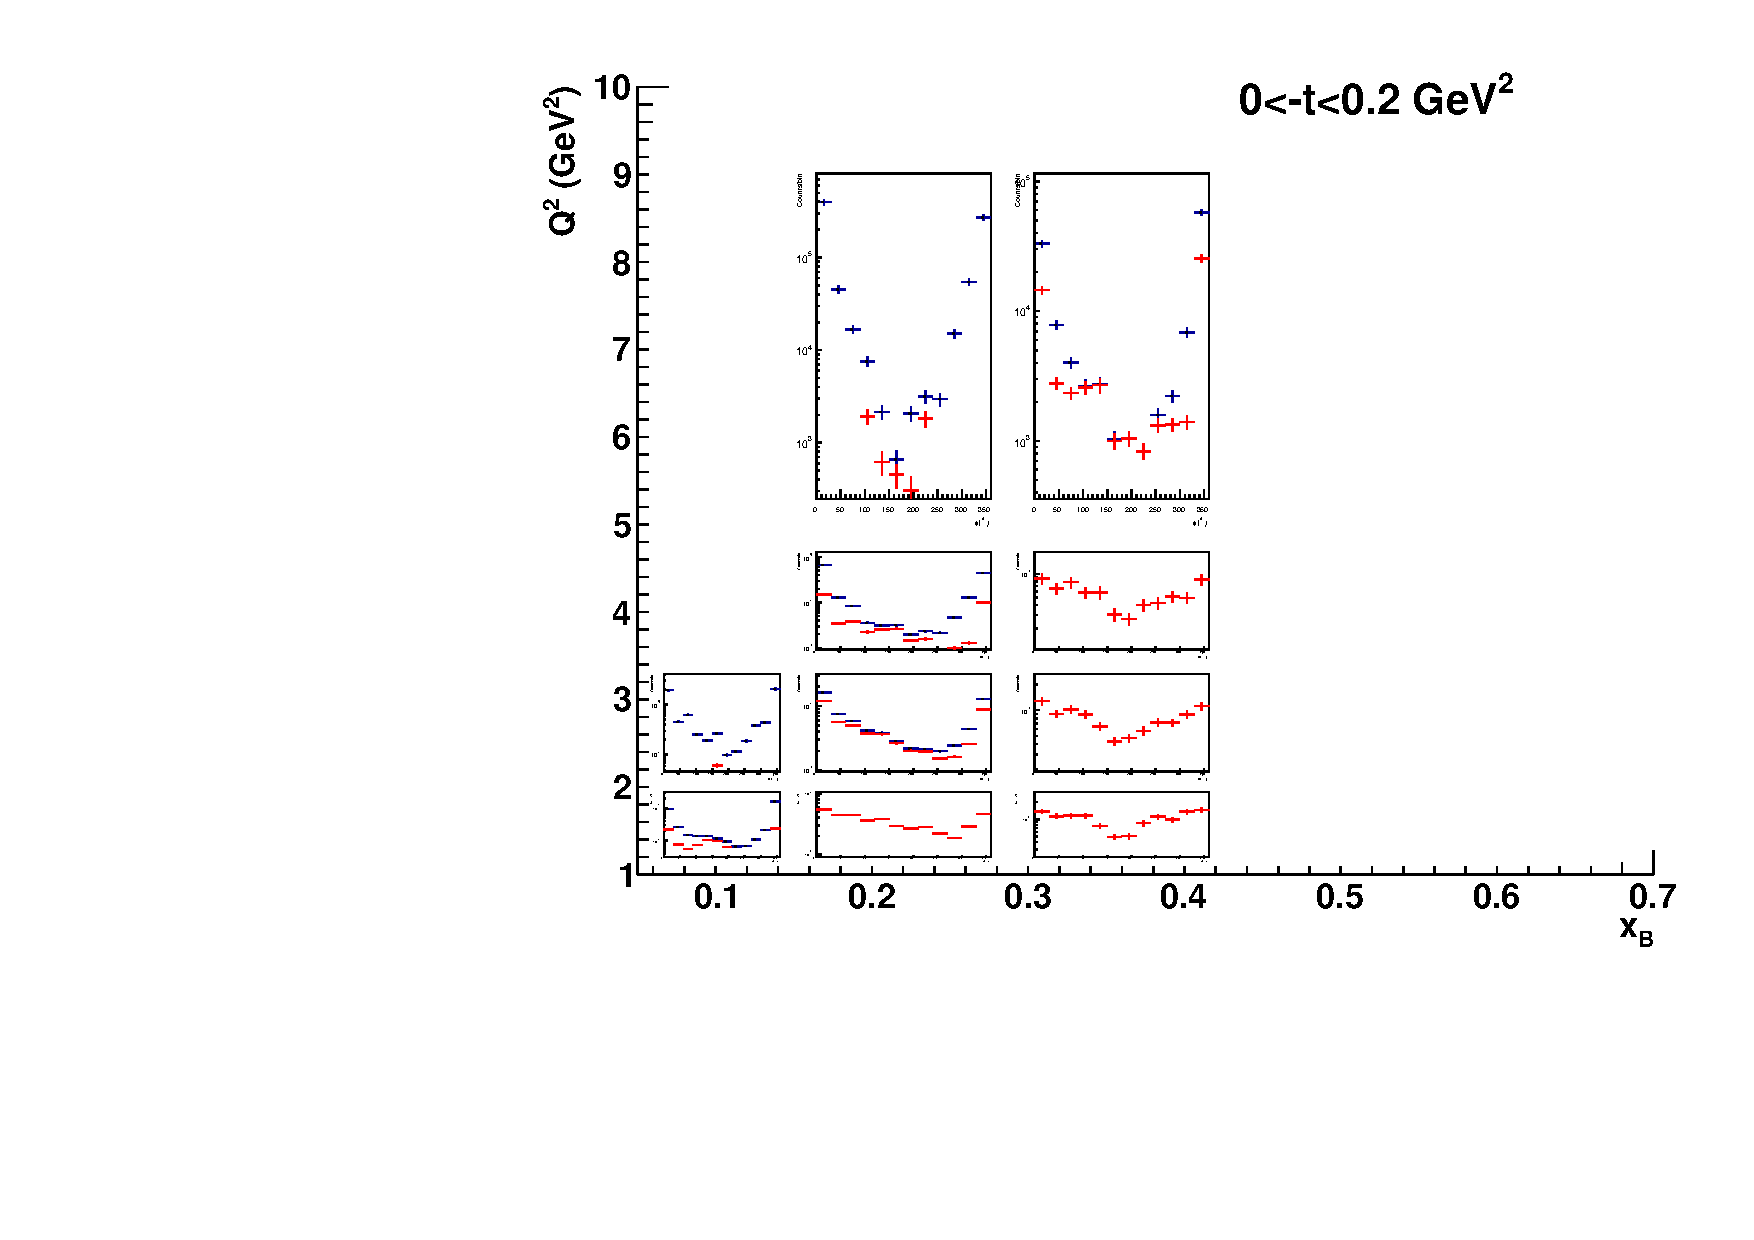
\includegraphics[width=130mm]{plot_counts_1_FT_noFT_100days.pdf}
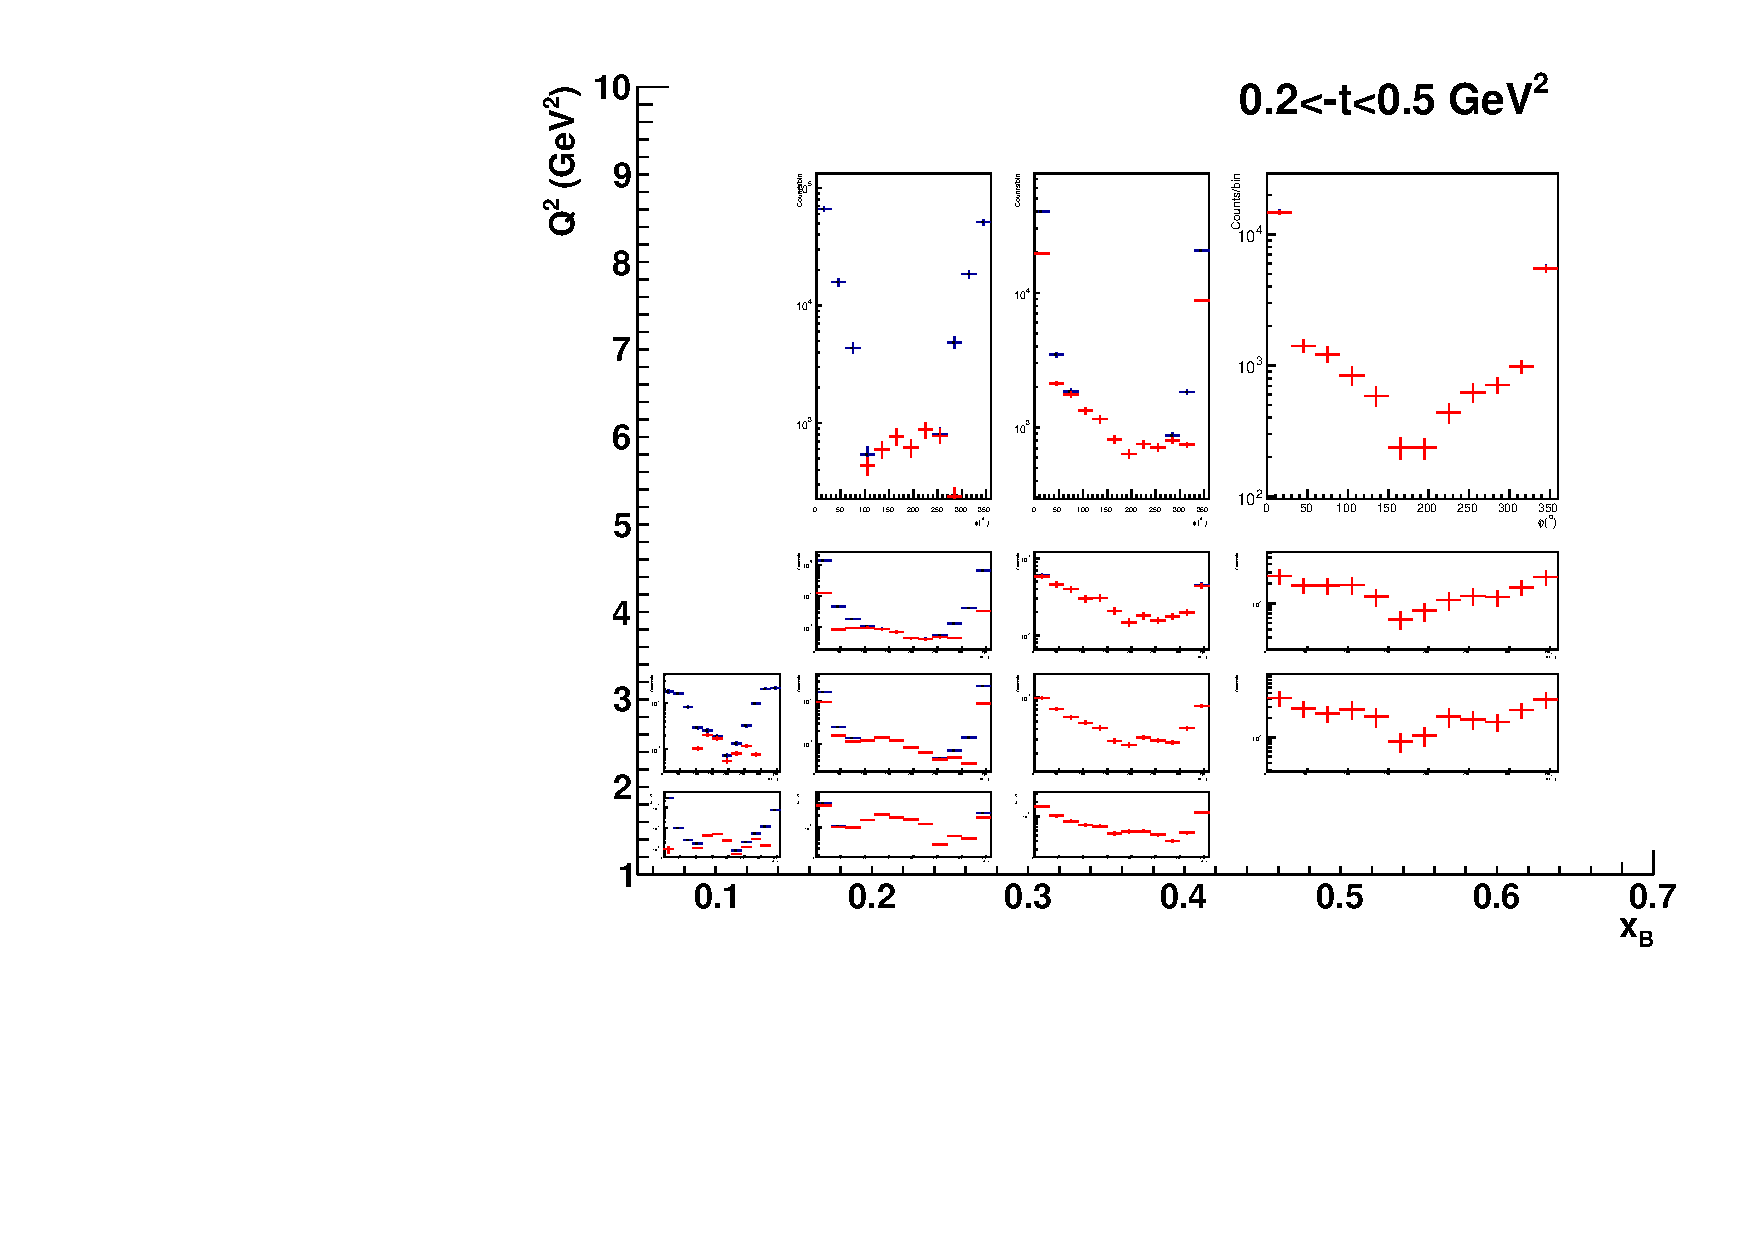
\includegraphics[width=130mm]{plot_counts_2_FT_noFT_100days.pdf}
\caption{Expected count rates for the nDVCS channel: $0.<-t<0.2$ GeV$^2$ (top) and $0.2<-t.0.5$ GeV$^2$ (bottom). Black: with FT; red: without FT. \label{count_rate_1}
}
\end{center}
\end{figure}
\begin{figure}  
\begin{center}
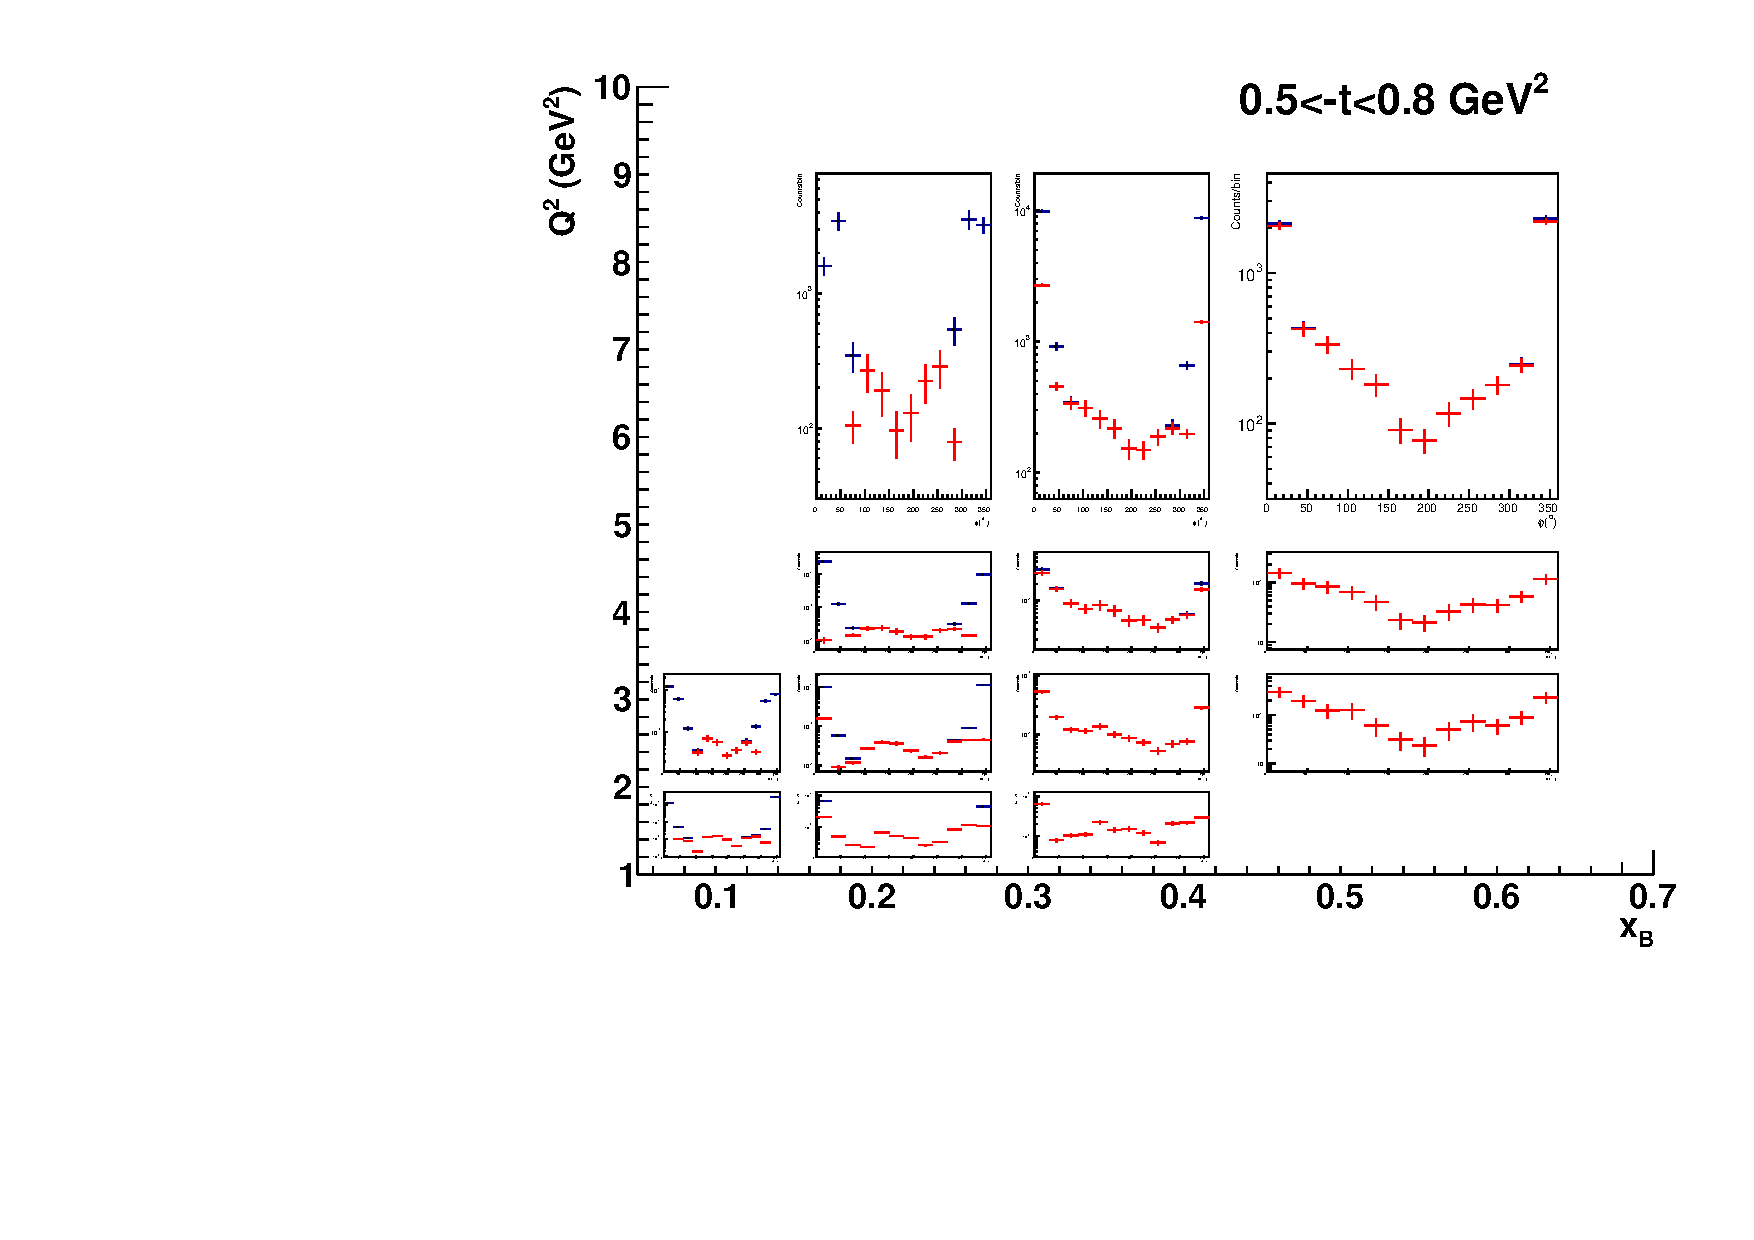
\includegraphics[width=120mm]{plot_counts_3_FT_noFT_100days.pdf}
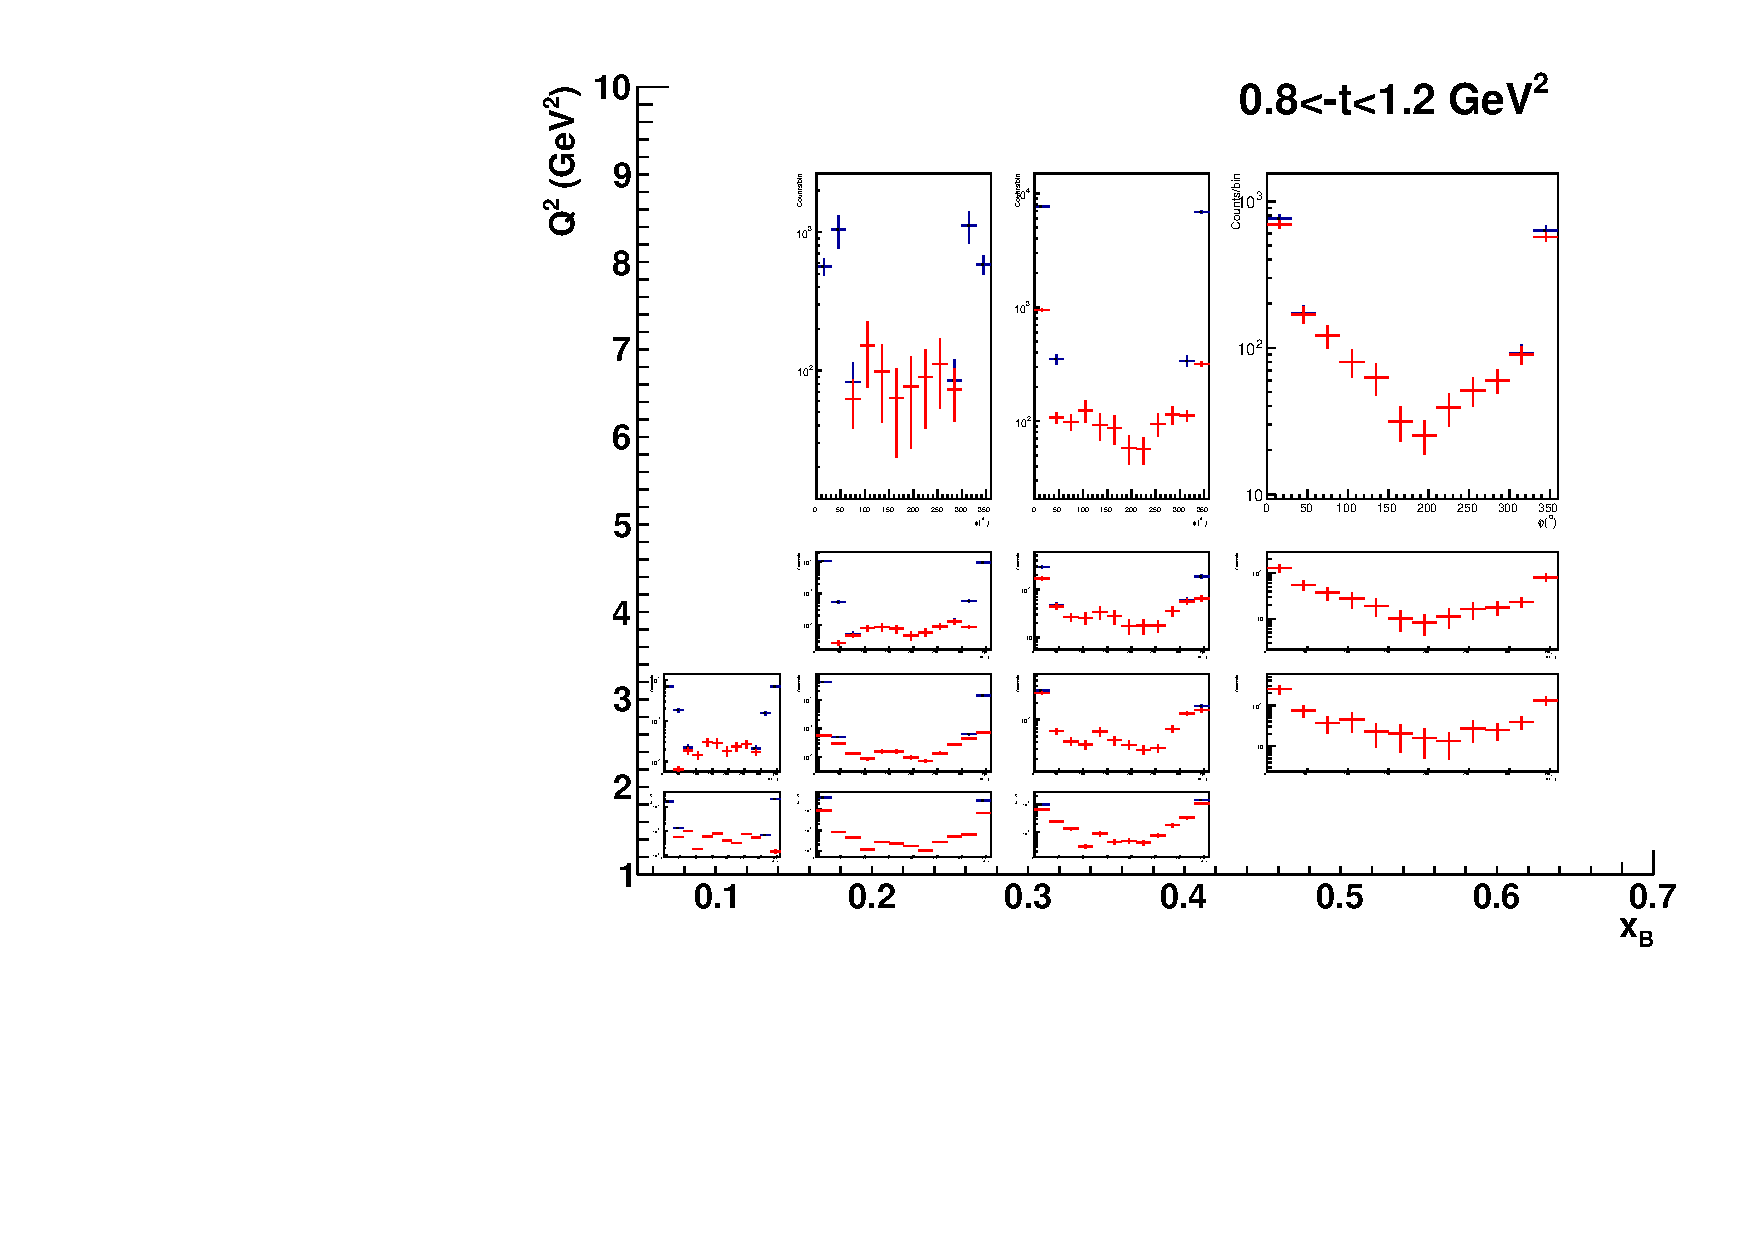
\includegraphics[width=120mm]{plot_counts_4_FT_noFT_100days.pdf}
\caption{Expected count rates for the nDVCS channel: $0.5<-t<0.8$ GeV$^2$ (top) and $0.8<-t<1.2$ GeV$^2$ (bottom). Black: with FT; red: without FT.\label{count_rate_2}}
\end{center}
\end{figure}

\begin{figure}  
\begin{center}
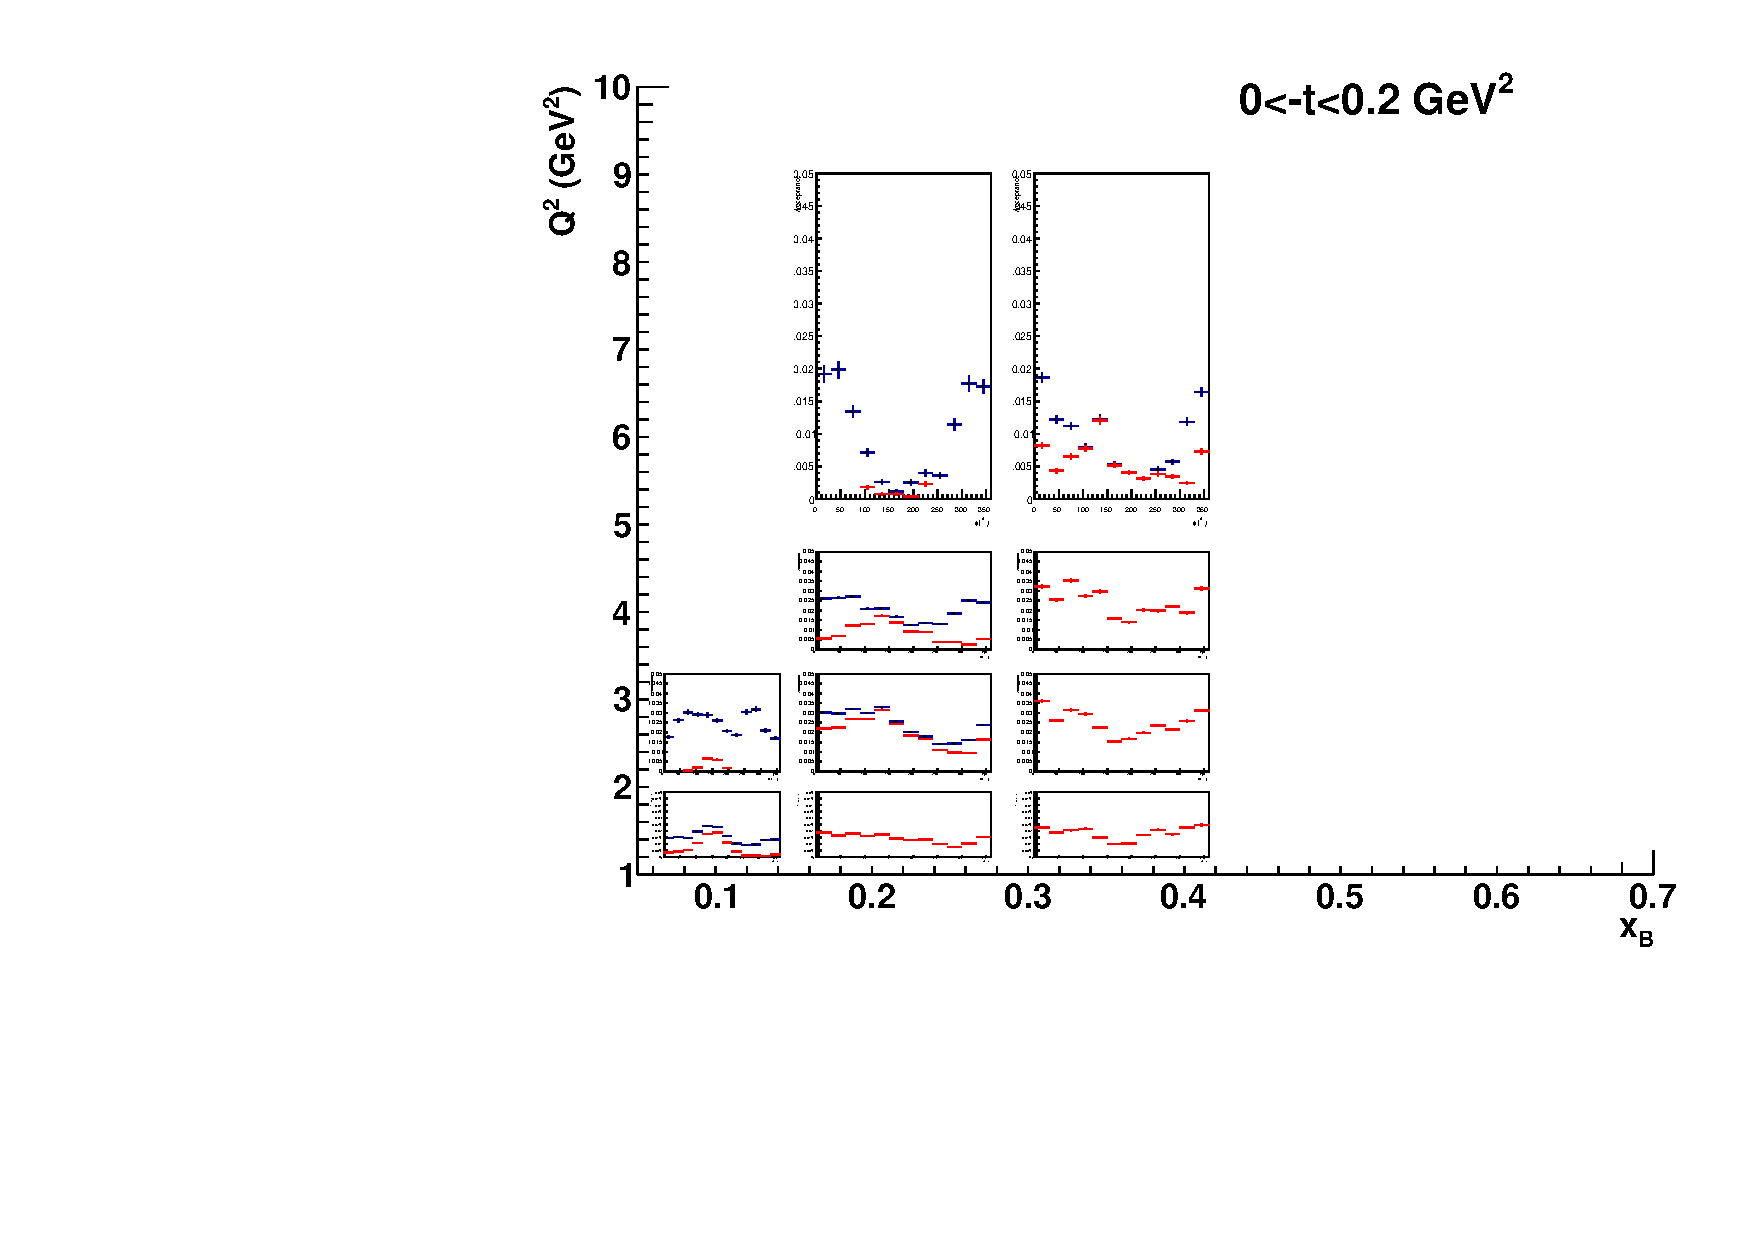
\includegraphics[width=130mm]{plot_acc_1_FT_noFT_100days.pdf}
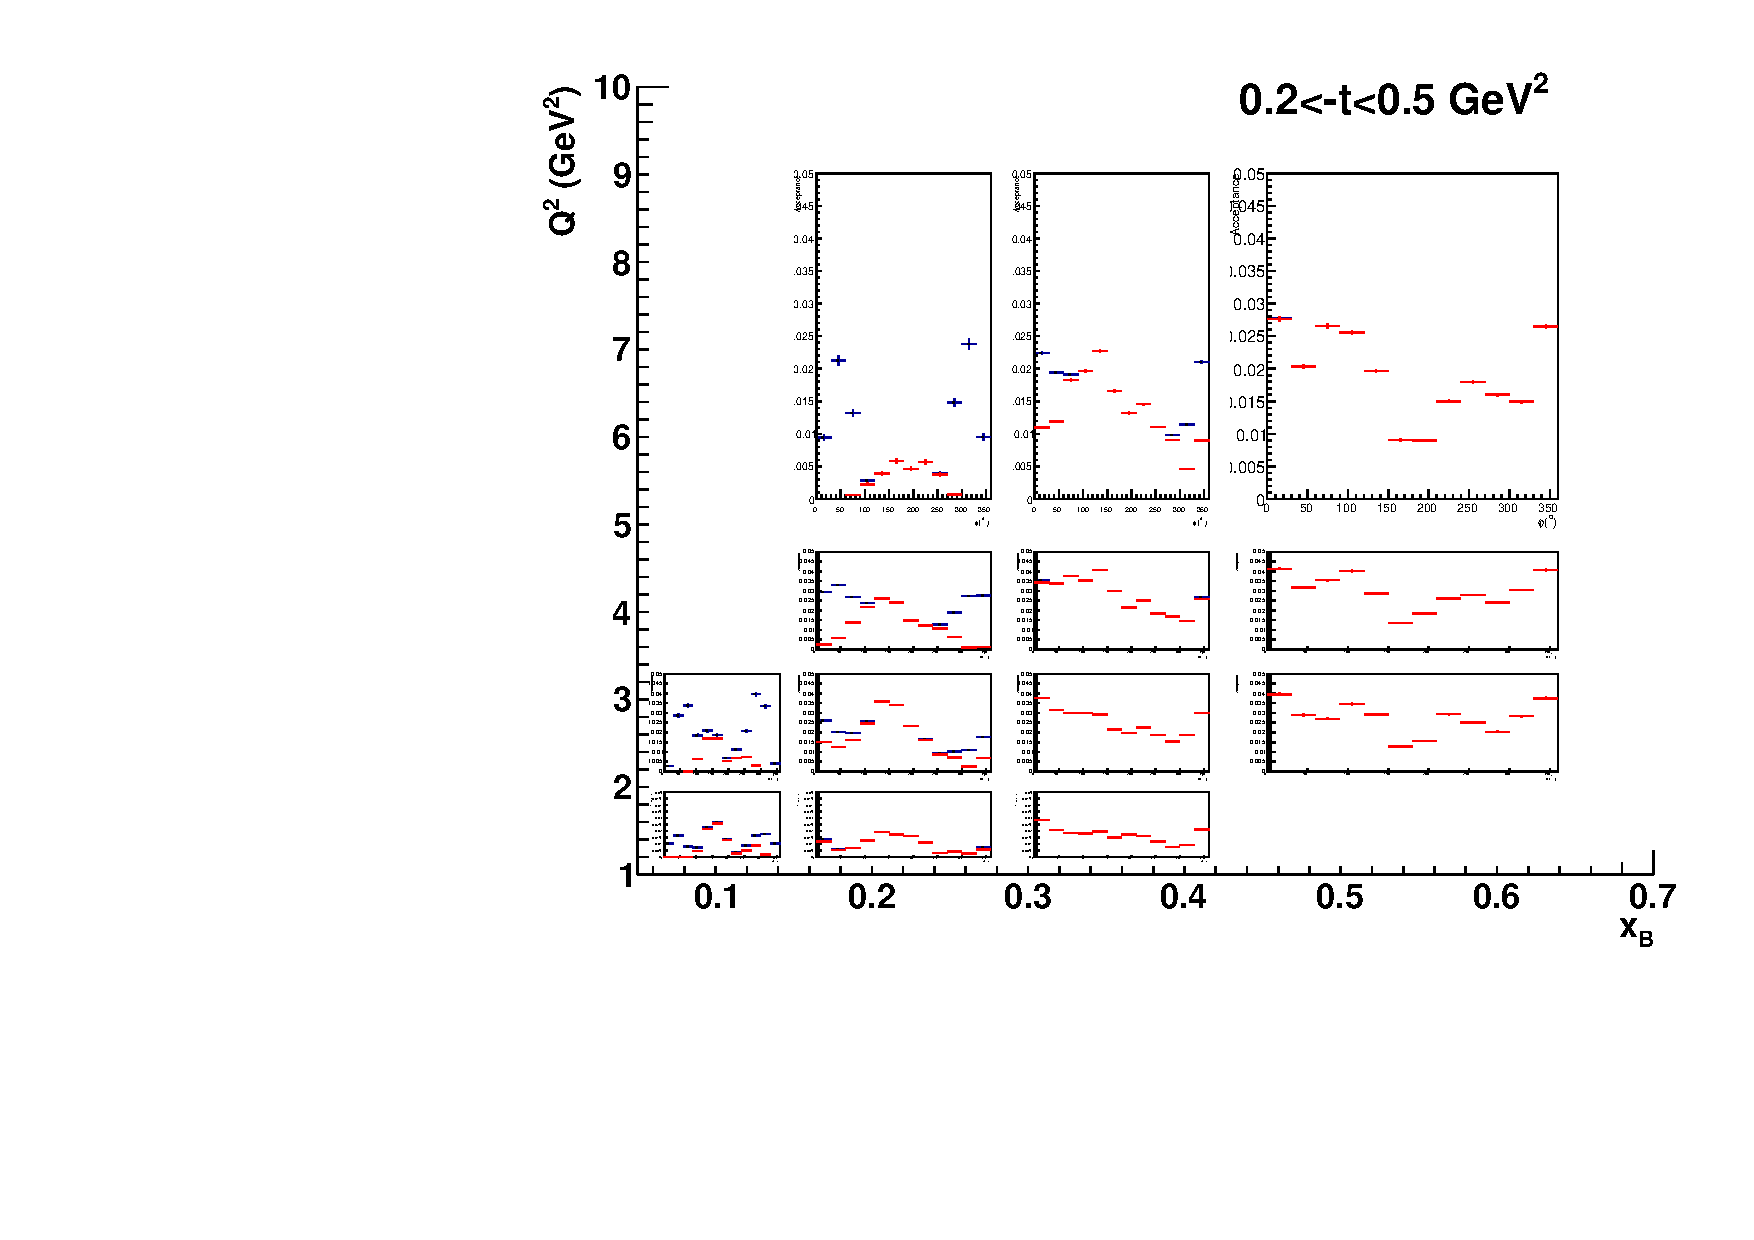
\includegraphics[width=130mm]{plot_acc_2_FT_noFT_100days.pdf}
\caption{Expected acceptances, including the 10\% of efficiency for the CND, for the nDVCS channel: $0.<-t<0.2$ GeV$^2$ (top) and $0.2<-t<0.5$ GeV$^2$ (bottom). All plots have $y$ scale ranging from 0 to 0.05 Black: with FT; red: without FT.. \label{acceptance_1}}
\end{center}
\end{figure}
\begin{figure}  
\begin{center}
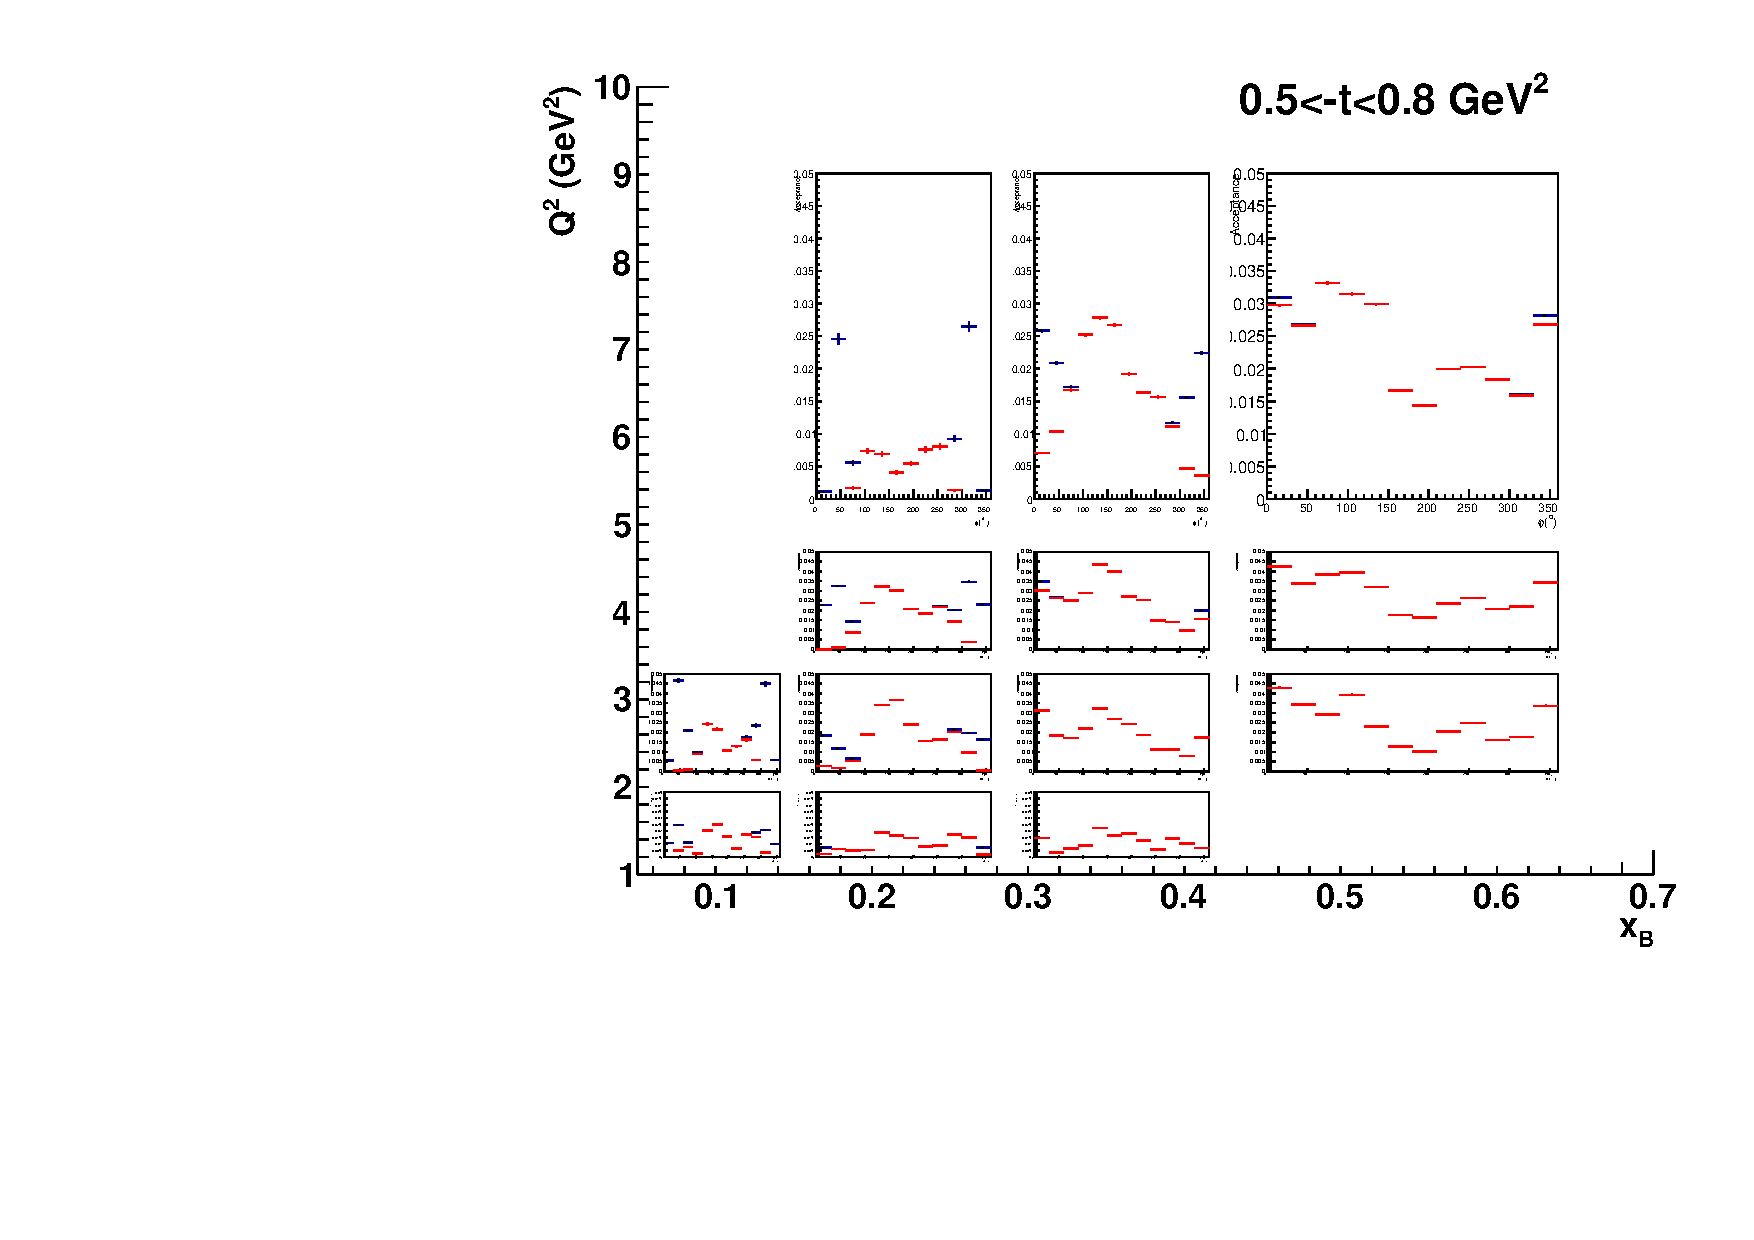
\includegraphics[width=120mm]{plot_acc_3_FT_noFT_100days.pdf}
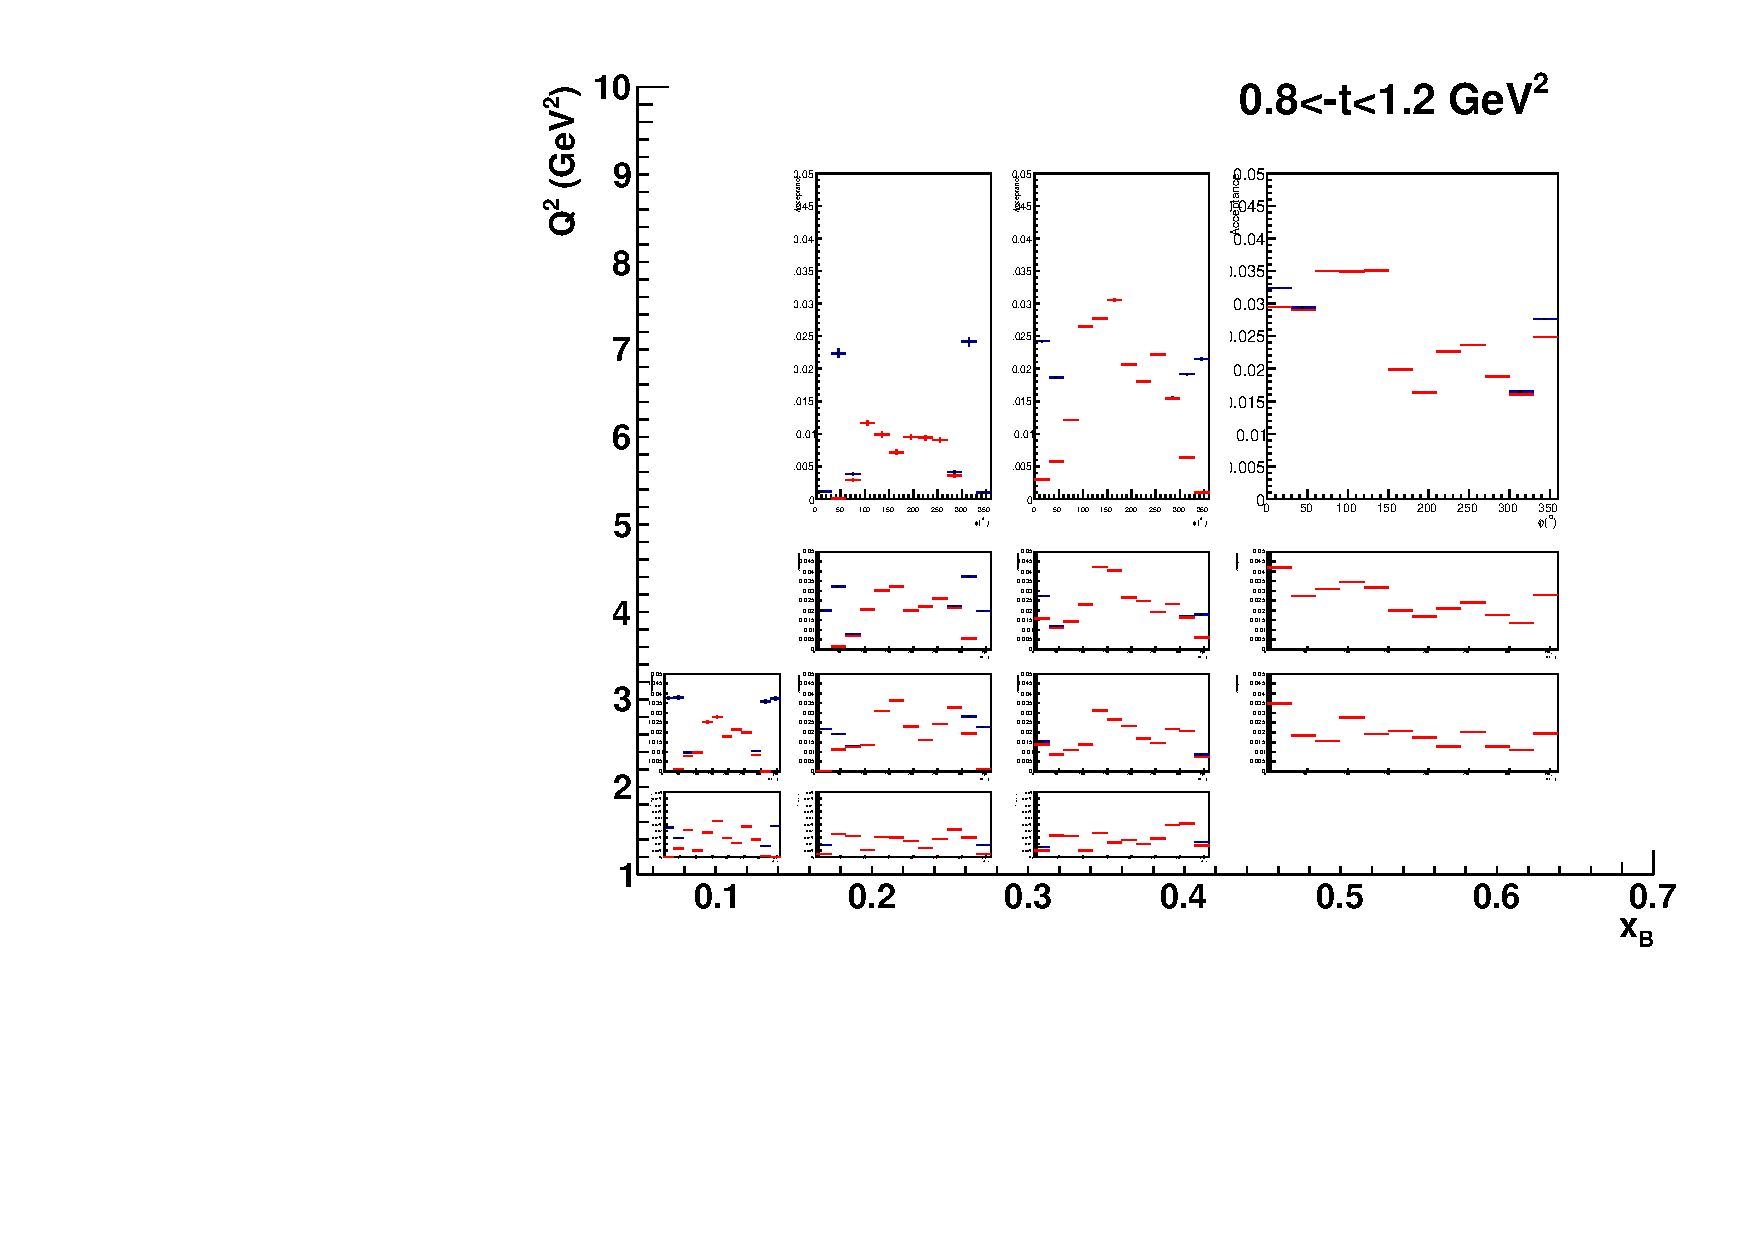
\includegraphics[width=120mm]{plot_acc_4_FT_noFT_100days.pdf}
\caption{Expected acceptances, including the 10\% of efficiency for the CND, for the nDVCS channel: $0.5<-t<0.8$ GeV$^2$ (top) and $0.8<-t<1.2$ GeV$^2$ (bottom). All plots have $y$ scale ranging from 0 to 0.05. Black: with FT; red: without FT. \label{acceptance_2}}
\end{center}
\end{figure}
